% This section includes some motivations behind the work, explicitly or implicitly highlights the research question , provides a high-level explanation of the solution, and describes the contributions.

% establish the context, background and/or importance of the topic
Historically, financial crime and transaction fraud have been a major concern in the business sector in the global economy. The number of fraud cases has increased drastically in recent times, affecting both financial institutions and their clients significantly. It has been found, from a recent survey done by PriceWaterhouse Coopers on economic crime and fraud, that the reported financial losses occurred between 2018 to 2020 is more than 42 billion dollars~\cite{PwC.Crime.Survey}. From the participated 5000 companies, it was calculated that On an average companies experienced 6 fraud cases during this period. Which refers that the actual number and amount of financial crime is way higher.   


Thirty five percent of the reported fraud cases during the mentioned period, faced by businesses in different sectors are marked as customer. An overview of customer fraud by sector is shown in the figure~\ref{fig:fraud_sector}  That means the majority of the financial crime faced by the business are done by their clients and business partners~\cite{PwC.Crime.Survey}. In recent trend to reduce operational cost and time, more and more, companies outsource non-core activities to third party companies. However, this cost saving activity imposes external fraud to the businesses from their party-party business partners and clients. On the flip side, suppliers and manufactures are in high risk of fraud cases from their clients and business partners. 


Hence, this is vital for the business to introduce a defence mechanism to prevent financial losses from external sources by applying internal process and system to detect suspicious clients and business partners. 

% brief synopsis of the relevant literature
% \subsection{What is Fraud?}\hspace*{\fill} \\
Fraud or extortion is a par of internal threats for any business. Manufacturers and service providers may face financial losses from fraudulent buyers. According to the Association of Certified Fraud Examiners (ACFE), the definition of fraud is \"the use of one’s occupation for personal enrichment through the misuse or deliberate misapplication of the resources or assets of the employing organization\"~\cite{kassem_2014}.

\begin{figure}[htp]
    \centering
    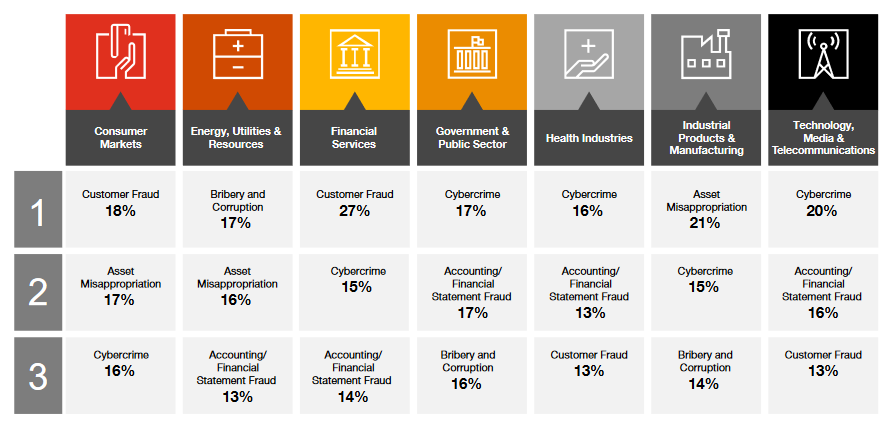
\includegraphics[width=\linewidth]{figures/fraud_by_industry.PNG}
    \caption{Most disruptive fraud events – by industry. Source: PwC 2020 Fraud survery~\cite{PwC.Crime.Survey} }
    \label{fig:fraud_sector}
\end{figure}
% Indicate an issue, problem or controversy in the field of study



A classical approach to preventing financial fraud by organizations is to incorporate operational processes to provide instructions to the employees for identifying anomalies and suspicious occurrences, which is then additionally governed by internal and external auditors. ~\cite{kassem_2014}. By following the operational processes, the employees try to find suspicious patterns through analyzing the transactions, financial statements, historical behaviour. 



Organizations and financial institutions use different technical solutions incorporated with their operational processes to verify their customers, vendors and business partners. Organizations use tools like Know your Customer (KYC) for customer onboarding, Anti-money laundering (AML) system for preventing financial crime, and internal reports for finding suspicious events. These processes are proven to be effective to detect suspicious events. However, the problems for these existing solutions are complex, time-consuming, costly, and cognitively challenging, and labour-intensive.


In the recent past with the advancement of data mining and machine learning technique, different machine learning-based solutions for detecting financial fraud are proven to be handy. ~\cite{RB2021, KIRKOS2007995}. Combining the machine learning-based solution with the existing operational process can help the organization reduce task complexity, operational cost, and human cognitive activities. 


Although lots of research has been carried out on detecting anomalies in financial crime, we can see that most of the researches for identifying suspicious financial crime activity are focused on detecting credit card fraud by using machine learning techniques~\cite{RB2021}.  However, as mentioned earlier, in the survey on financial crime and fraud done by PwC, we have seen that third party business crime and fraud imposes high risk and have significant financial losses for the organizations.

% listing the research question or hypotheses


This paper will focus on using a data-driven approach using machine learning techniques to detect suspicious companies to prevent financial losses for the organizations and respective financial institutions. The main objective of this study is a) to use a data mining technique to extract features from unstructured data and b) apply ensemble learning and neural networks to identify the patterns on the engineered features to classify suspicious companies. 

% provide synopsis of the research methods


Previous studies have reported (see section~\ref{sec: related work}) the effectiveness of using data driven machine learning approaches in real world data. Due to the complexity of the problems each real world data needs to be handled based on its merit. However using data driven approach generally leads to finding the suitable information for the models. 





% Significance of value of the study


This thesis provided an important opportunity to advance the understanding of data-driven approach for extrapolate data from historical archive based on expert opinion. Also the paper covers how a real-world data with high class imbalanced is used for different machine learning approaches. The paper also tries to explain the complexity and challenges of identifying anomalies in the data set and share a practical overview on how to approach suspicious recommendation engine can be applied this financial and other suitable sectors.



% Define the topic or key term


Throughout this paper, the term provider is referred to the trade credit insurance provider. The term client is referred as the client of the insurance service provider or suppliers. The term buyers are the clients of the suppliers. Credit insurance also referred as policy in the paper. 

% Overview of teh report stucture
\subsubsection{Structure:}\hspace*{\fill} \\
To overall structure of the design takes the form of three steps. In step 1 a data driven technique is used to identify the most significant information based on the feedback from expert then extracting the information from historical dataset. In step 2 ensemble models and neural networks are used for suspicious companies classification problem. And last but not least, in step 3 Different machine learning metrics are used to select the best performing model. The details of the approach are described in the overview [section: ~\ref{sec: Overview}] and design [sec:~\ref{sec: Design}] section of this paper.

\begin{itemize}
    \item[a.] Data driven approach to extract relevant information related to detecting suspicious behaviour or patters of companies
    \item[b.] Building ensemble learning and neural networks models for pattern recognition. 
    \item[c.] Choosing the most appropriate model for detecting suspicious companies to prevent fraudulent cases.
\end{itemize}


% State the purpose of the essay / write


The case study of identifying suspicious companies that presented in this paper is conducted for one of the leading trade insurance company. The interested company has foot print over different locations in the world. The target of the company to reduce risk by preparing a classification model which recommends or detects suspicious companies to prevent itself from having financial loss due to fraudulent activity.
% Provide an overview of the coverage

\subsubsection{Limitation:}\hspace*{\fill} \\
Designing and setting the suitable machine learning model is a repetitive process. In this paper only section method of first model is described. Due to practical constrain not all other machine learning models and configuration of assembly models and neural networks are discussed. Also due to protect the internal process of the expertise of the insurance company have been excluded while describing the feature. However in the design section a generalized approach and pseudo code have been shared in section:~\ref{sec: Design}]






